\documentclass[a4paper,12pt]{article}

% don't forget the document class, generally : \documentclass[a4paper,12pt]{article}

\usepackage[utf8]{inputenc}
\usepackage[french]{babel}
\usepackage{graphicx}
\usepackage{gensymb}
\usepackage{amsmath}
\usepackage{float}
\usepackage{scrextend}
\usepackage{caption} 
\usepackage{siunitx}
\usepackage{enumitem}
\usepackage{amsthm}
\usepackage{fancyhdr}
\usepackage{amssymb}
\usepackage{wrapfig}
\usepackage{geometry}
\usepackage{standalone}
\usepackage{import}
\usepackage[usenames, dvipsnames]{color}

 \usepackage{biblatex} % manages bibliography and references
\addbibresource{sample.bib}


\geometry{hmargin=1in, vmargin=1in}

 \newenvironment{absolutelynopagebreak}
 {\par\nobreak\vfil\penalty0\vfilneg
 \vtop\bgroup}
 {\par\xdef\tpd{\the\prevdepth}\egroup
 \prevdepth=\tpd}
 
 \pagestyle{fancy}                        
\fancyhf{}                               
\fancyhf[HL]{Application des maths}                
\fancyhf[HR]{Géométrie euclidienne}             
\fancyhf[FC]{\thepage/\pageref{Lastpage}}
 
\newtheorem{definition}{Définition}[section]
\newtheorem{theorem}{Théorème}
\newtheorem{corollary}{Corollaire}[theorem]
\newtheorem{lemma}[theorem]{Lemme}
\newtheorem*{hyp}{Hypothèse}
\newtheorem*{concl}{Conclusion}
\newtheorem*{remark}{Remarque}

\captionsetup{format=default,labelformat=simple,labelsep=colon,
justification=justified,font={sf,small},labelfont=bf,
textfont=default} 



\begin{document}

\pagebreak
\subsubsection{Théorème 3 (théorème de Thalès)}
\begin{theorem}
Deux paires de parallèles qui découpent sur une droite deux segments proportionnels découpent des segments de mèeme proportion sur toute sécante de la première droite.
\end{theorem}

\begin{proof}
Nous considérons le triangle quelconque $ABC$ 
\begin{hyp}

\begin{itemize}
    \item $m$ et $m'$ deux droites, $m \cap m'$
    \item $a$, $b$ $c$ et $d$ sont quatre droites parallèles qui interceptent $m$ et $m'$ respectivement en $A$, $B$, $C$ et $D$ et $A'$, $B'$, $C'$ et $D'$.
\end{itemize}

\end{hyp}

\begin{concl}
$\frac{AB}{CD} = \frac{A'B'}{C'D'}$
\end{concl}
\begin{figure}[H]
        \centering
        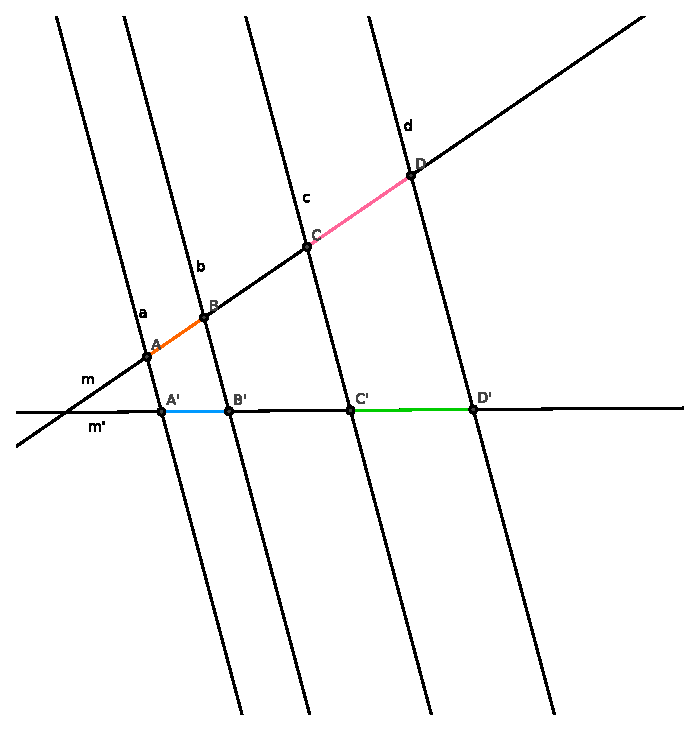
\includegraphics[scale=1.2]{thales1.eps}
    \end{figure}

\begin{remark}
Notre démonstration ne peut être utilisée qu'avec des nombres rationnels. En effet, celle pour les nombres réels est bien plus complexe et nous ne l'aborderons pas.
\end{remark}

Afin de démontrer ce théorème pour les nombres rationnels, nous exprimons le ratio $\frac{AB}{CD}$ sous une forme rationnelle, c'est-à-dire sous forme $\frac{p}{q}$. Nous réalisons la démonstration avec $\frac{AB}{CD} = \frac{3}{5}$, une valeur numérique, afin de faciliter la compréhension de la démonstration.\\

Nous commençons par diviser $AB$ en trois parties isométriques et $CD$ en cinq. Nous nommons respectivement $EF$ et $GH$ un des segments ainsi formés.
Ainsi nous obtenons que $AB = 3EF$ et $CD = 5EF$. Donc $\frac{3EF}{5GH} = \frac{AB}{CD} = \frac{3}{5}$ et l'on observe que $EF \equiv GH$.\\

\begin{figure}[H]
        \centering
        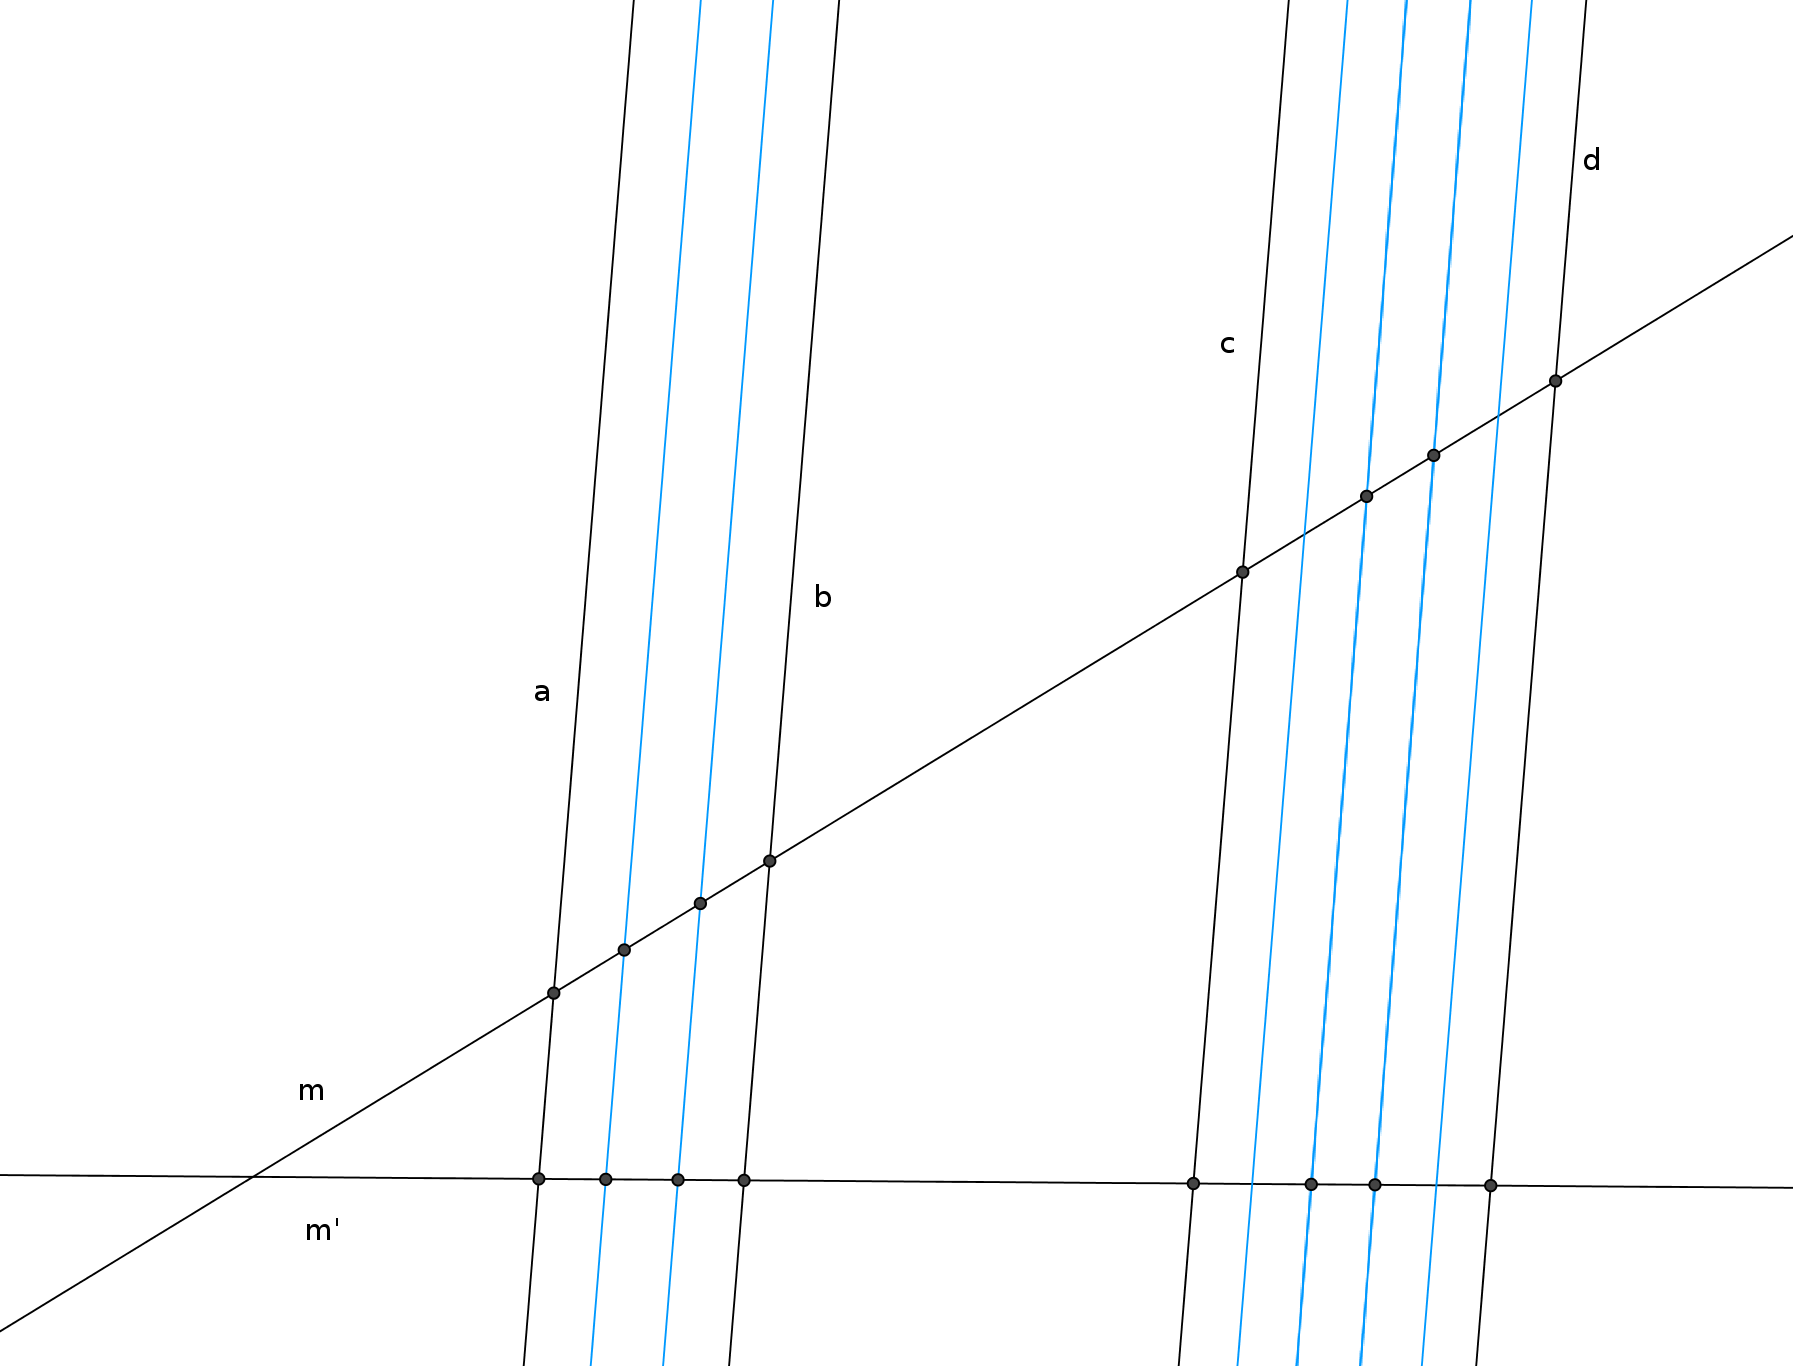
\includegraphics[scale=1.1]{thales2.png}
    \end{figure}

 Dès lors, si l'on trace des droites parallèles aux premières et passant par les points $E$, $F$, $G$ et $H$, l'on sait que les segments qu'elles découpent sur $m'$ sont isométriques (grâce au théorème précédent, théorème \ref{semblableTh2}). Nommons deux de ces segments $E'F'$ et $G'H'$, alors $\frac{AB}{CD} = \frac{3}{5} = \frac{3E'F'}{5G'H'} = \frac{A'B'}{C'D'}$.
Ainsi, si on généralise cette démonstration à $\frac{A'B'}{C'D'} = \frac{p}{q}$, on démontre le théorème de Thalès pour tous les nombre rationnels.
\end{proof}




\pagebreak
\begin{remark}
Thalès vécu au septième et sixième siècle avant J.C. dans la ville de Milet, en Grèce. Marchand de profession, il est aussi philosophe et l'un des précurseurs de la pensée scientifique moderne. En effet, au lieu de reposer l'explication de phénomènes inexpliqués sur la mythologie, il privilégia l'observation et son expérience personnelle. Ce procédé lui permit de faire de nombreuses découvertes et inventions d'une grande importance, notamment en astronomie, physique et mathématiques.\\
\begin{figure}[H]
    \centering
    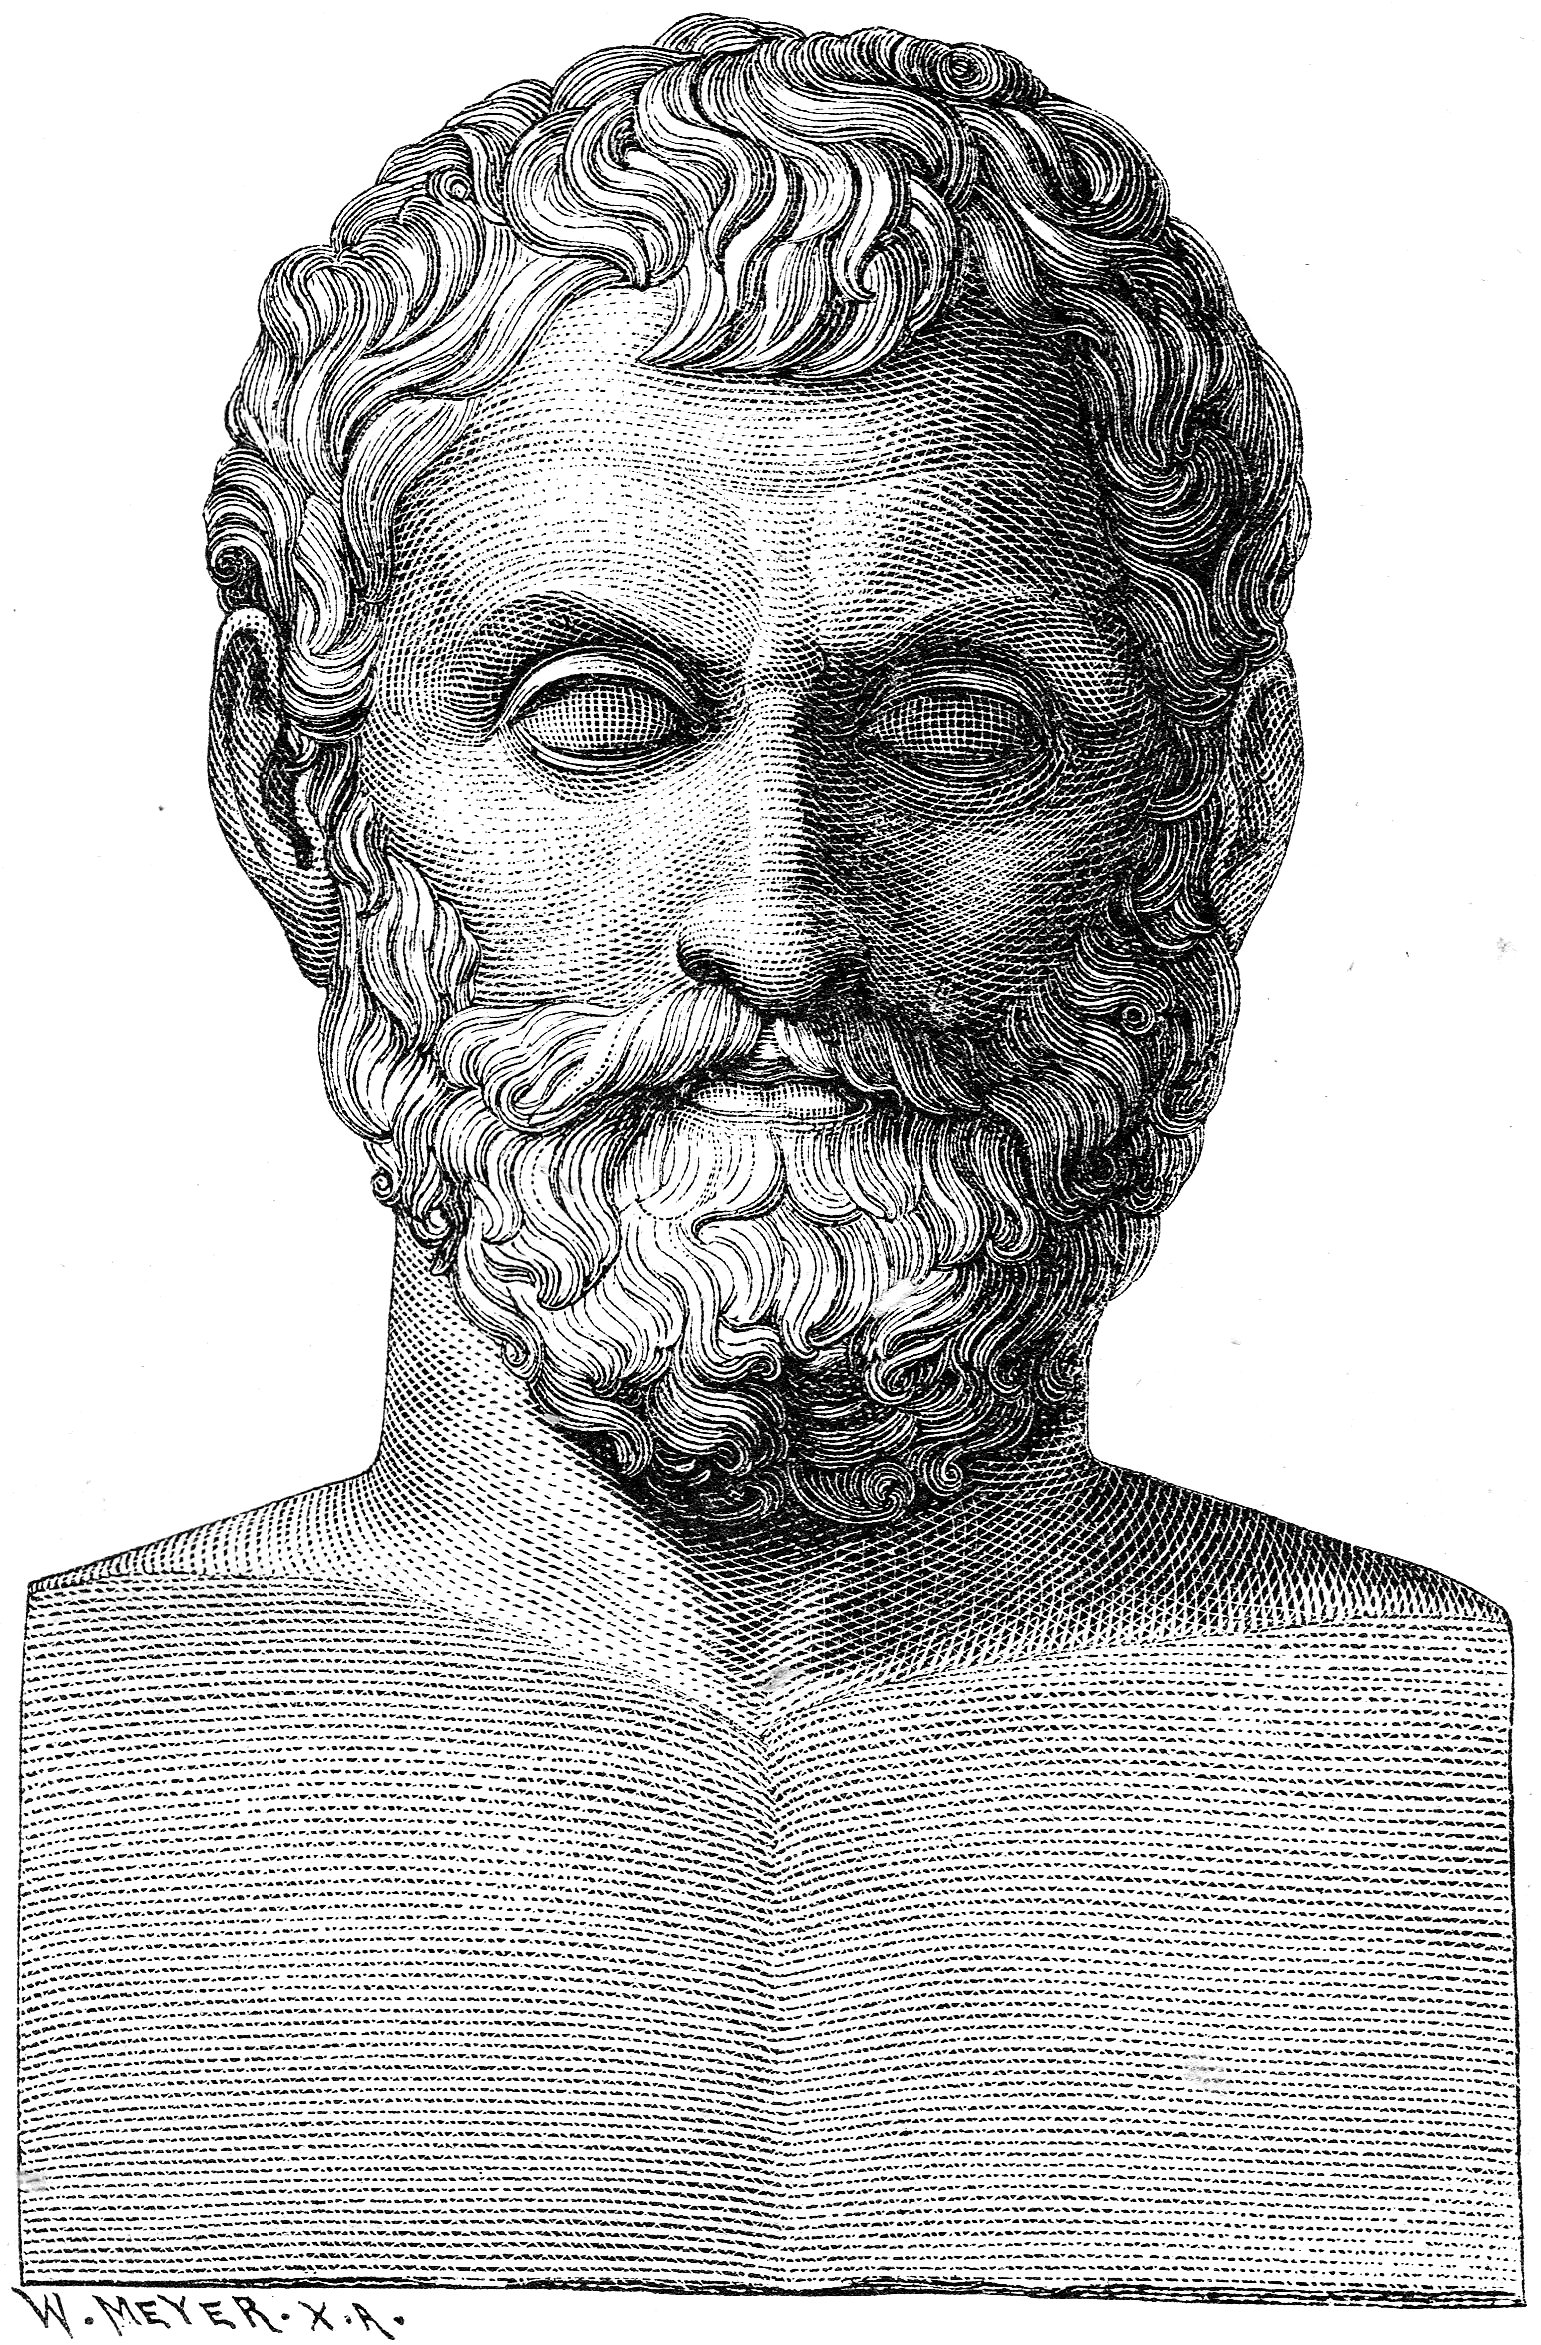
\includegraphics[scale = 0.2]{theorems/semblables/thales/thales.jpg}
    
    \caption{Portrait de Thalès de Milet}
    \label{fig:thales}
\end{figure}

\pagebreak
On lui accorde, entre autre, la découverte d'un moyen de mesurer la hauteur des pyramides d'Egypte. Il observa qu'il existe chaque jour un moment lors duquel un objet et son ombre ont la même longueur. Par conséquent, lors d'une journée où les rayons du soleil sont perpendiculaires à un des côtés de la base de la pyramide (ce qui arrive deux fois par an), la hauteur de la pyramide sera égale à la longueur de son ombre à cette heure précise, à laquelle on additionne la moitié de la longueur du côté de la pyramide. Cette expérience est résumée sur le schéma ci-dessous (figure \ref{fig:exp}\footnote{Wikimedia, File: Thales Theorem 6.svg, Fred the Oyster, 20.11.2016}).
\footnote{Inspiré du site web Bibm@th.net, article "Thalès de Milet (624 av JC - 547 av JC)", 20.11.2016, disponible:
http://www.bibmath.net/bios/index.php?action=affiche\&quoi=thales et de Wikipedia, article "Thalès", 20.11.2016, disponible: https://fr.wikipedia.org/wiki/Thal\%C3\%A8s\#cite\_note-61}


\begin{figure}[H]
    \centering
    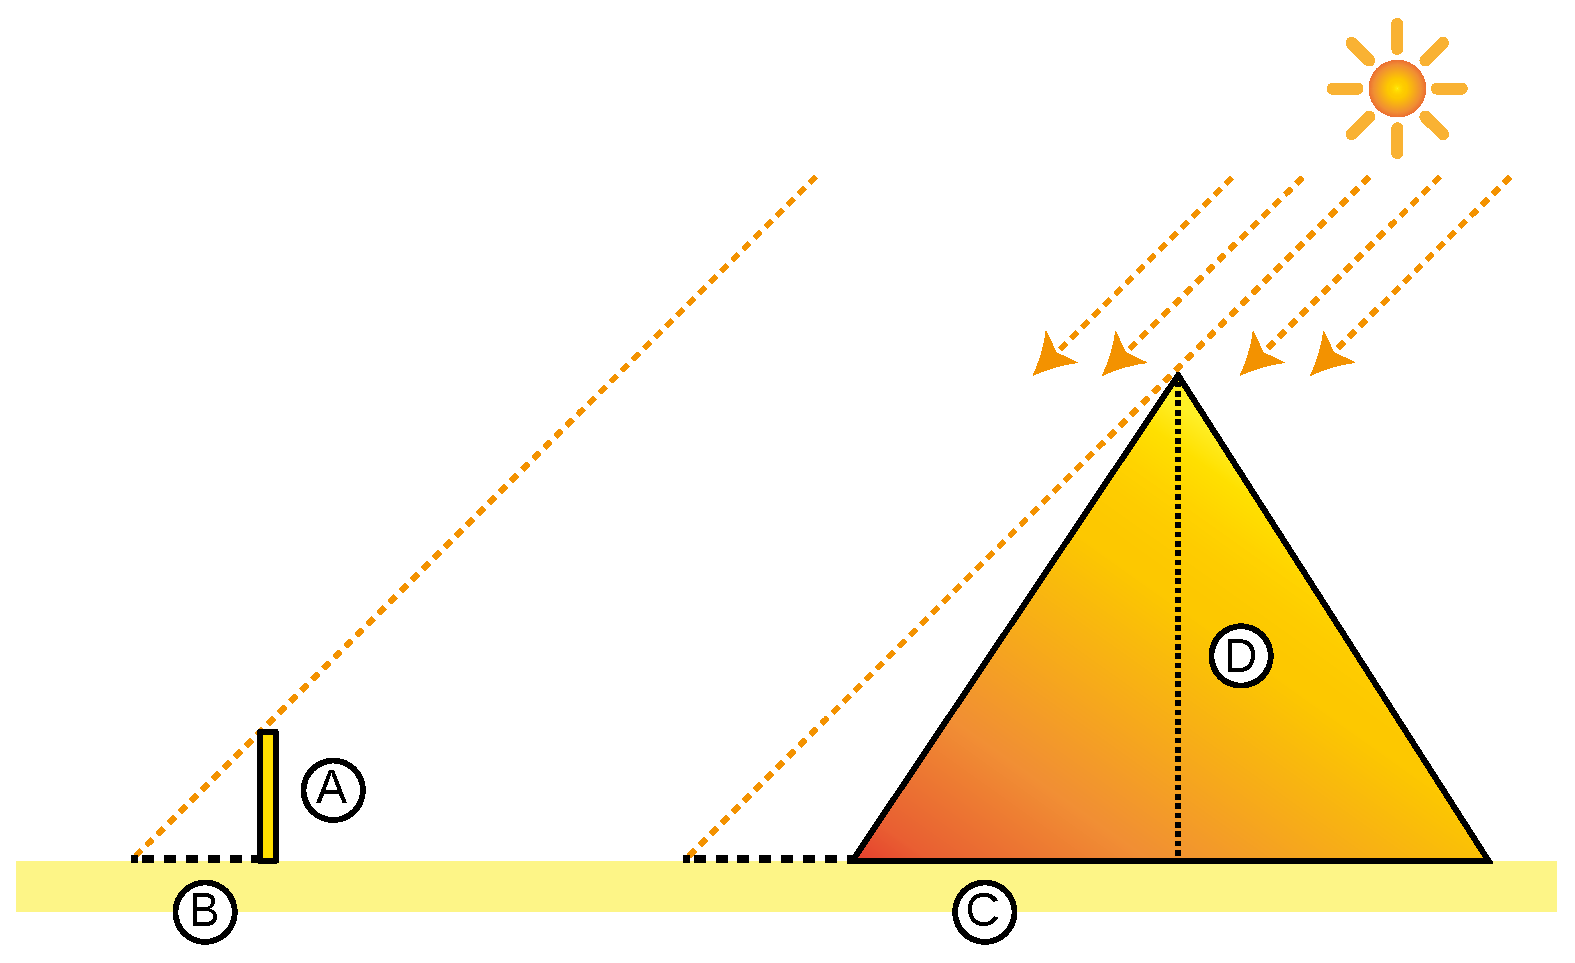
\includegraphics[width=\textwidth]{theorems/semblables/thales/Thales_Theorem_6.eps}
    
    \caption{}
    \label{fig:exp}
\end{figure}
\end{remark}

\end{document}
